% ==========================================
% PHỤ LỤC B: ĐÁNH GIÁ LUỒNG XỬ LÝ HAI GIAI ĐOẠN
% ==========================================
\chapter{ĐÁNH GIÁ LUỒNG XỬ LÝ HAI GIAI ĐOẠN}
\label{AppendixB}

Phụ lục B đánh giá ảnh hưởng của lỗi sàng lọc lên kết quả phân đoạn cuối cùng, khi đặt PGA-UNet phía sau một bước sàng lọc tự động là Gatekeeper, tức là một mô hình EfficientNet-B3~\cite{tan2019efficientnet} dùng để phân loại ảnh bình thường và bất thường, thì lỗi ở bước sàng lọc sẽ tác động thế nào đến kết quả phân đoạn cuối cùng. Gatekeeper ở đây không phải là đóng góp kiến trúc chính của khóa luận. Phần này cũng không nhằm chứng minh hiệu năng của một hệ thống chẩn đoán tự động hoàn chỉnh, mà chỉ xem lỗi sàng lọc ảnh hưởng như thế nào đến toàn bộ luồng xử lý khi chưa có bác sĩ chẩn đoán ảnh can thiệp lại.
% ------------------------------------------------------------
\section{Kết quả trên BTXRD}
\label{subsec:product_overview_btxrd}
% ------------------------------------------------------------

\subsection{Hiệu năng của Gatekeeper}
\label{sec:danh_gia_phan_lop}

Gatekeeper sử dụng EfficientNet-B3 được tiền huấn luyện trên ImageNet-1K và tinh chỉnh cho bài toán phân loại nhị phân. Mô hình nhận ảnh kích thước $300\times300$ và trả về xác suất bất thường, ngưỡng phân loại mặc định được đặt tại 0,5.

Mô hình được đánh giá trên tập ảnh hỗn hợp gồm 375 ảnh kiểm thử của BTXRD, trong đó có 187 ảnh bệnh lý và 188 ảnh bình thường. Kết quả được trình bày trong Bảng~\ref{tab:classification_results}.

\needspace{12\baselineskip}
\begin{table}[htbp]
    \centering
    \caption{Kết quả phân loại của Gatekeeper trên BTXRD}
    \label{tab:classification_results}
    \renewcommand{\arraystretch}{1.3}
    \begin{tabular}{|p{7.5cm}|c|}
        \hline
        \textbf{Chỉ số} & \textbf{Kết quả} \\
        \hline
        Accuracy & 87,73\% \\
        \hline
        Precision & 86,53\% \\
        \hline
        Sensitivity & 89,30\% \\
        \hline
        Specificity & 86,17\% \\
        \hline
        F1-score & 87,90\% \\
        \hline
        AUC-ROC & 0,9421 \\
        \hline
    \end{tabular}
\end{table}

AUC-ROC 0,9421 và Accuracy 87,73\% cho thấy Gatekeeper phân biệt khá tốt hai loại ảnh trên BTXRD. Nhưng ở ngưỡng mặc định 0,5, vẫn có 20/187 ảnh bệnh lý bị bỏ sót (Sensitivity 89,30\%), nên chưa thể dùng Gatekeeper như một bộ lọc tự động loại bỏ ảnh lành lặn mà không có ai xem lại.

\subsection{Ảnh hưởng đến luồng phân đoạn}
\label{sec:pipeline_eval}
\label{subsec:cascading_error}

Để khảo sát ảnh hưởng của lỗi sàng lọc, thực nghiệm mô phỏng trường hợp kết quả Gatekeeper được sử dụng trực tiếp mà không có bước kiểm tra lại của bác sĩ chẩn đoán ảnh. Trong 187 ảnh bệnh lý, 167 ảnh được chuyển đúng sang PGA-UNet và 20 ảnh bị loại nhầm. Hộp giới hạn của các ảnh được tạo từ chú thích gốc của nhãn nhằm giữ cố định chất lượng câu nhắc, sau đó mới chuyển sang quá trình phân đoạn; do đó, thực nghiệm tập trung vào lỗi sàng lọc của Gatekeeper, không đánh giá khả năng tự động tạo hộp giới hạn.

Trên 167 ảnh bệnh lý được chuyển đúng, PGA-UNet đạt Dice trung bình 0,8626. Để biểu diễn ảnh hưởng của sai số tích lũy, khóa luận sử dụng Dice toàn luồng có phạt lỗi sàng lọc: ảnh được chuyển đúng đóng góp Dice phân đoạn thực tế, trong khi ảnh bệnh lý bị bỏ sót và ảnh bình thường bị chuyển nhầm được gán giá trị 0. Chỉ số này được xác định bởi:

\begin{equation}
    \mathrm{Dice}_{\mathrm{pipeline}}
    =
    \frac{
        \displaystyle\sum_{i\in\mathrm{TP}}
        \mathrm{Dice}_{\mathrm{img}}(i)
    }{
        N_{\mathrm{TP}}+N_{\mathrm{FP}}+N_{\mathrm{FN}}
    }.
    \label{eq:pipeline_dice}
\end{equation}

Với 167 TP, 26 FP và 20 FN, Dice toàn luồng đạt 0,6763. Bảng~\ref{tab:pipeline_eval} tóm tắt kết quả.

\needspace{12\baselineskip}
\begin{table}[htbp]
    \centering
    \caption{Kết quả mô phỏng luồng xử lý hai giai đoạn trên BTXRD}
    \label{tab:pipeline_eval}
    \renewcommand{\arraystretch}{1.3}
    \begin{tabular}{|p{8cm}|c|}
        \hline
        \textbf{Thống kê} & \textbf{Giá trị} \\
        \hline
        Tổng số ảnh & 375 \\
        \hline
        TP / FP / FN / TN & 167 / 26 / 20 / 162 \\
        \hline
        Dice của PGA-UNet trên ảnh TP & 0,8626 \\
        \hline
        Dice toàn luồng có phạt lỗi sàng lọc & \textbf{0,6763} \\
        \hline
    \end{tabular}
\end{table}

Trong trường hợp không có bác sĩ chẩn đoán ảnh nào kiểm tra lại quyết định của Gatekeeper, tức là xét trong kịch bản xấu nhất chứ không phải quy trình thật đã đề xuất ở Chương~\ref{Chapter3}, thì Dice toàn luồng giảm từ 0,8626 xuống 0,6763. Phần giảm 0,1863 này đến từ cả hai loại lỗi sàng lọc: 26 ảnh bình thường bị chuyển nhầm và 20 ảnh bệnh lý bị bỏ sót, cả hai đều bị tính là 0 trong công thức trên. Trong hai loại này, ảnh bệnh lý bị bỏ sót vẫn đáng ngại hơn về mặt lâm sàng, vì đó là ca bệnh không bao giờ đến được PGA-UNet. Nhìn chung, mô hình phân đoạn vẫn hoạt động ổn định; vấn đề chính nằm ở bước sàng lọc phía trước.

Trong quy trình đề xuất tại Chương~\ref{Chapter3}, Gatekeeper chỉ cung cấp gợi ý sàng lọc và bác sĩ chẩn đoán ảnh vẫn xác nhận trước khi chuyển sang bước tiếp theo. Vì chưa thực hiện thử nghiệm có sự tham gia của bác sĩ trong thực tế, kết quả trên chỉ phản ánh kịch bản mô phỏng không có hiệu chỉnh của con người, không đại diện cho hiệu năng lâm sàng của hệ thống hoàn chỉnh.

Hình~\ref{fig:qual_pipeline_tp} minh họa một số ảnh bệnh lý được Gatekeeper phát hiện đúng và chuyển sang PGA-UNet. Các trường hợp này cho thấy mô hình có thể tiếp tục phân đoạn tổn thương tại nhiều vị trí giải phẫu khi ảnh được sàng lọc đúng và cung cấp câu nhắc phù hợp.

\needspace{14\baselineskip}
\begin{figure}[htbp]
    \centering
    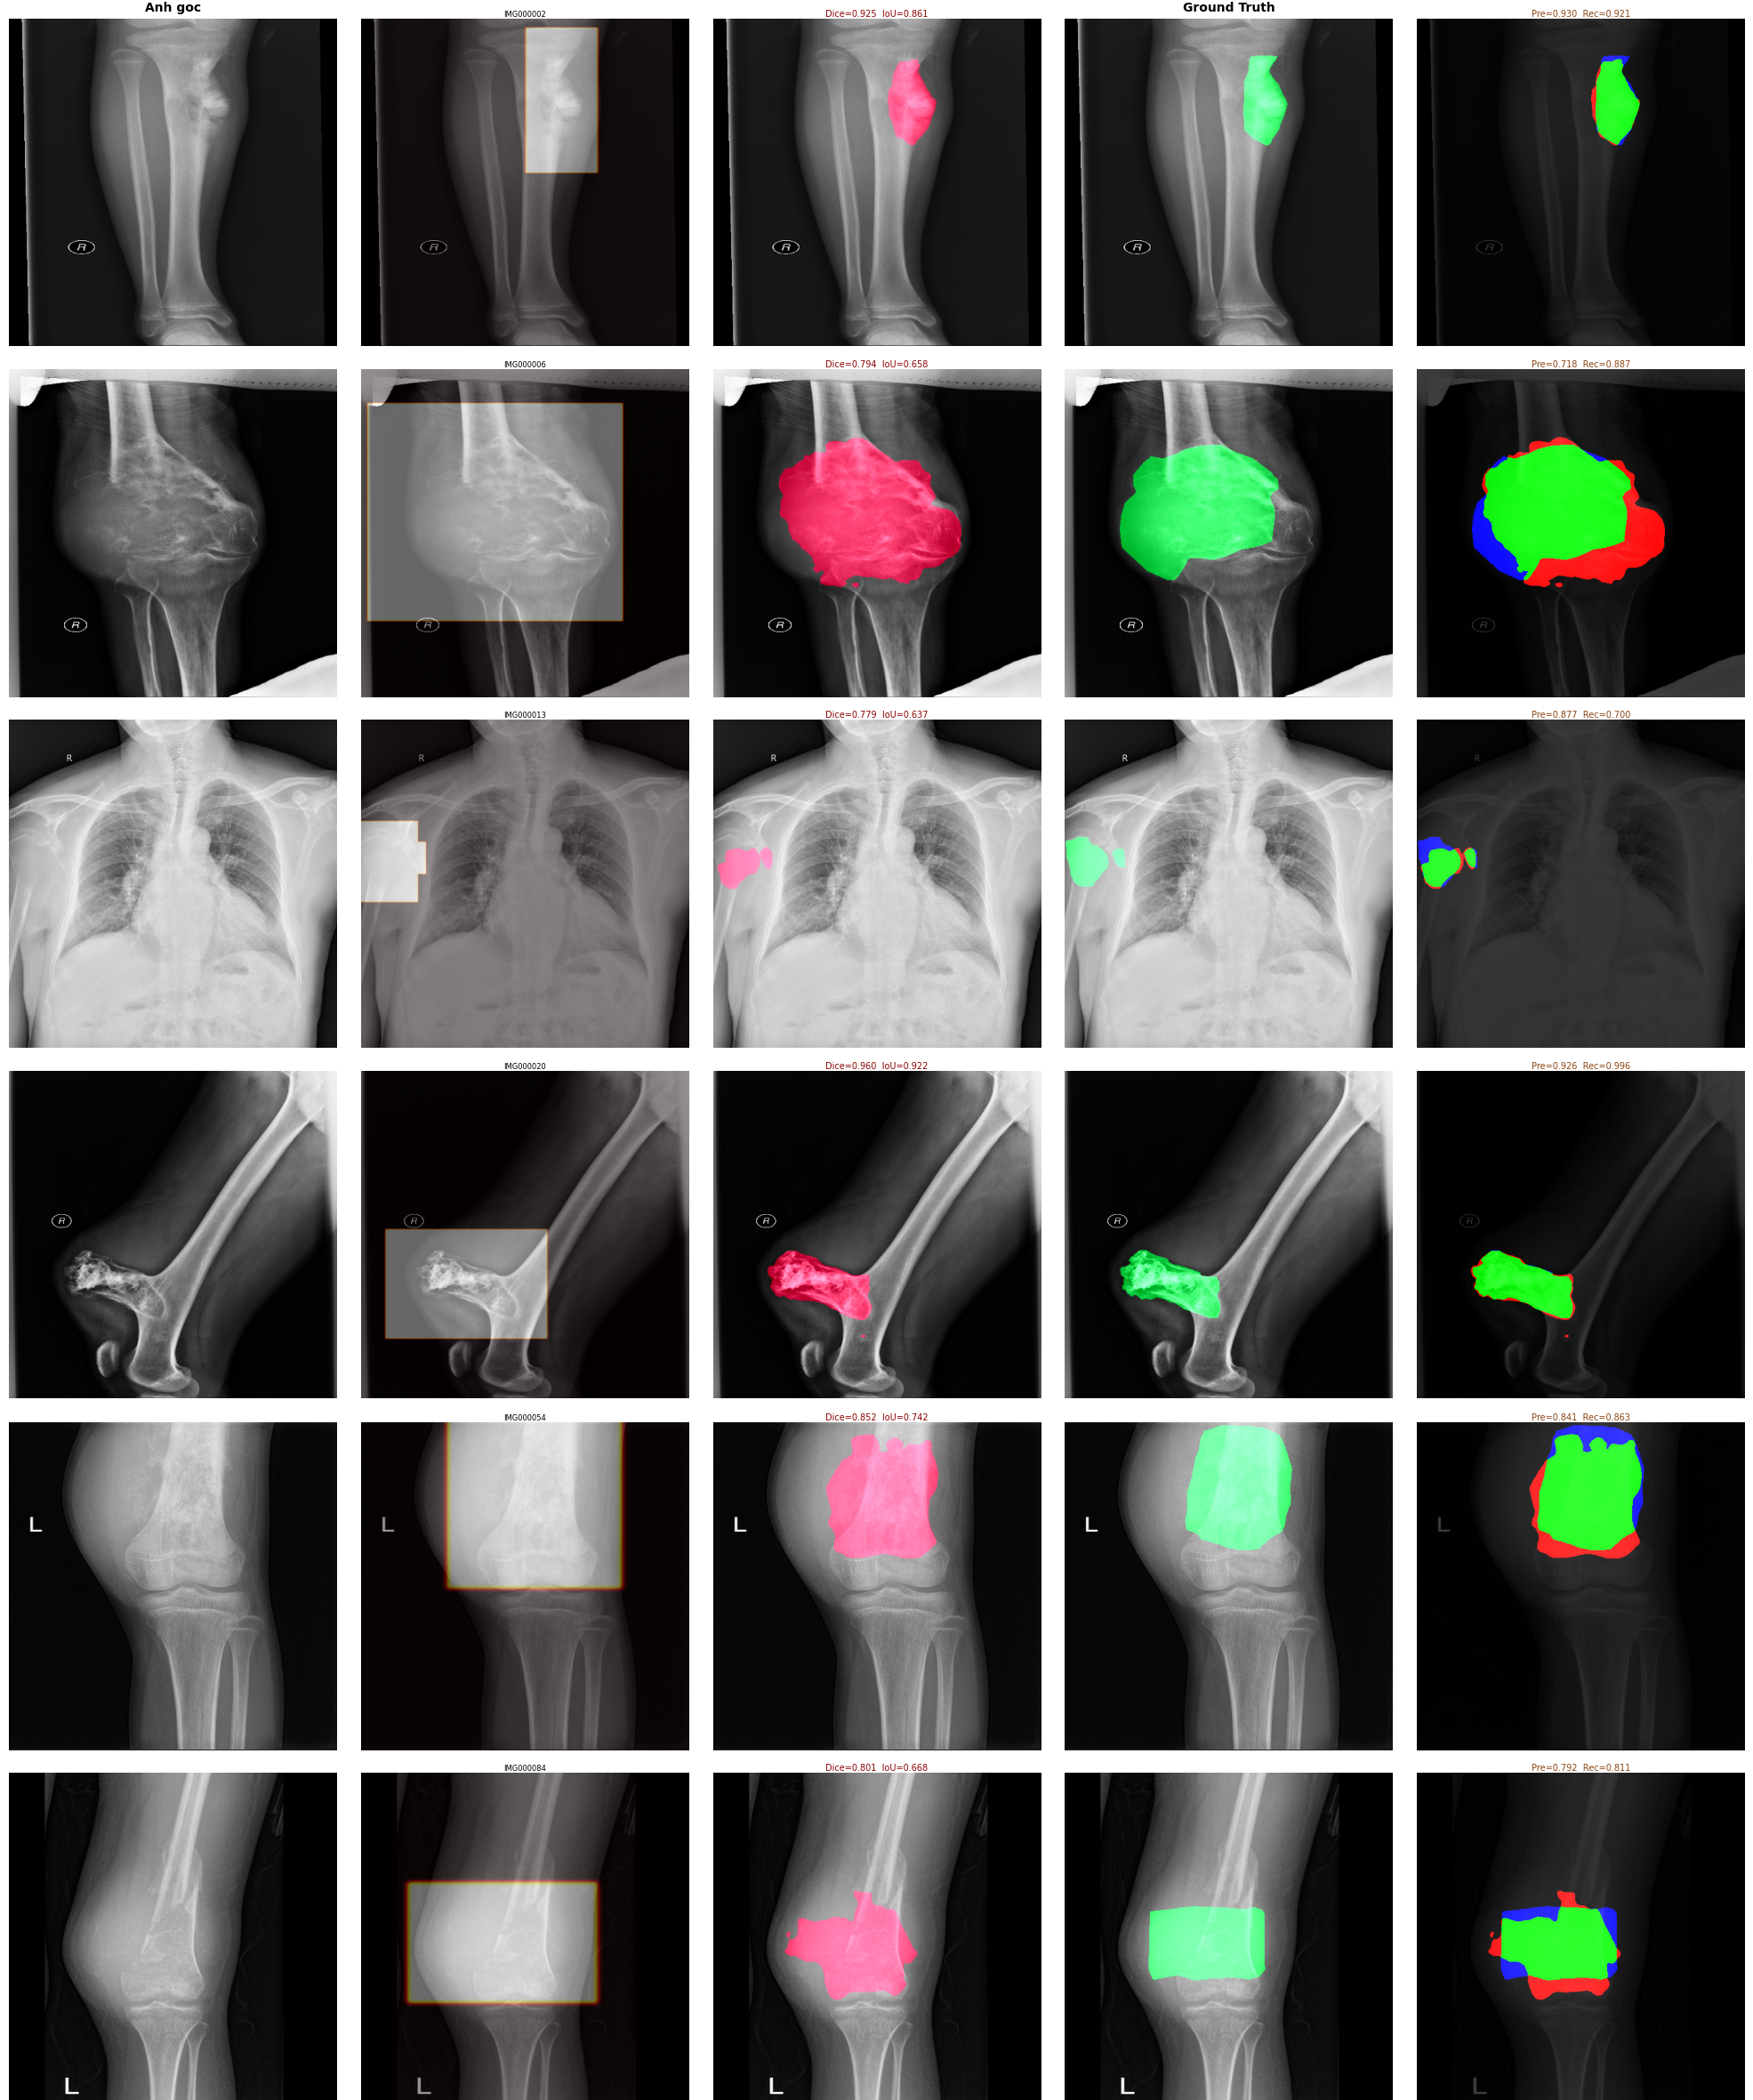
\includegraphics[width=0.65\textwidth]{images/qual_pipeline_tp.png}
    \caption{Một số kết quả phân đoạn của ảnh được Gatekeeper phân loại đúng và chuyển sang PGA-UNet trên BTXRD. Từ trái sang phải: ảnh X-quang, hộp giới hạn, mặt nạ dự đoán, mặt nạ nhãn gốc và lớp phủ TP, FP, FN.}
    \label{fig:qual_pipeline_tp}
\end{figure}

\noindent\textbf{Kết luận}\\
Gatekeeper có thể hỗ trợ sàng lọc ảnh đầu vào, nhưng sai số tại bước này có thể làm giảm hiệu năng của toàn bộ luồng xử lý. Vì vậy, kết quả không làm thay đổi vai trò trung tâm của PGA-UNet mà chỉ cho thấy một điều kiện cần để triển khai mô hình trong thực tế: Gatekeeper nên được dùng như công cụ hỗ trợ, còn quyết định cuối cùng và cung cấp câu nhắc vẫn cần bác sĩ chẩn đoán ảnh xác nhận.

% ------------------------------------------------------------
\section{Kết quả trên FracAtlas}
\label{subsec:product_overview_fracatlas}
% ------------------------------------------------------------

Gatekeeper giữ nguyên kiến trúc EfficientNet-B3 và quy trình huấn luyện như trên BTXRD, nhưng được huấn luyện lại hoàn toàn trên FracAtlas. Thực nghiệm này nhằm kiểm tra khả năng tích hợp PGA-UNet vào cùng một luồng xử lý trên dữ liệu gãy xương, không đánh giá khả năng suy luận trực tiếp giữa hai miền dữ liệu.

\subsection{Hiệu năng của Gatekeeper}
\label{subsec:gatekeeper_fa}

Gatekeeper được đánh giá trên 409 ảnh kiểm thử của tập FracAtlas, gồm 72 ảnh gãy xương và 337 ảnh bình thường. Tỉ lệ này gần với phân bố của bộ dữ liệu gốc và mất cân bằng hơn rõ rệt so với tập kiểm thử của tập BTXRD.

\needspace{12\baselineskip}
\begin{table}[htbp]
    \centering
    \caption{Kết quả phân loại của Gatekeeper trên FracAtlas}
    \label{tab:classification_results_fa}
    \renewcommand{\arraystretch}{1.3}
    \begin{tabular}{|p{7.5cm}|c|}
        \hline
        \textbf{Chỉ số} & \textbf{Kết quả} \\
        \hline
        Accuracy & 88,26\% \\
        \hline
        Precision & 65,38\% \\
        \hline
        Sensitivity & 70,83\% \\
        \hline
        Specificity & 91,99\% \\
        \hline
        F1-score & 68,00\% \\
        \hline
        AUC-ROC & 0,9132 \\
        \hline
    \end{tabular}
\end{table}

AUC-ROC vẫn khá (0,9132), nhưng Sensitivity rơi xuống 70,83\%, tức là 21/72 ảnh bệnh lý bị bỏ sót. Ngược lại, 310/337 ảnh bình thường được xác định đúng, tương ứng Specificity 91,99\%. Có thể thấy trên dữ liệu mất cân bằng, mô hình nghiêng nhiều hơn về phía dự đoán bình thường, đồng thời cũng khó nhận diện các đường gãy nhỏ và mảnh hơn.

\subsection{Ảnh hưởng đến luồng phân đoạn}
\label{subsec:pipeline_eval_fa}

Luồng xử lý được đánh giá trên toàn bộ 409 ảnh kiểm thử theo cùng thiết lập tại Mục~\ref{sec:pipeline_eval}. Kết quả của Gatekeeper được sử dụng trực tiếp mà không có bước kiểm tra lại của bác sĩ chẩn đoán ảnh. Đối với ảnh bệnh lý được chuyển đúng sang PGA-UNet, hộp giới hạn của các ảnh được tạo từ chú thích gốc của nhãn nhằm giữ cố định chất lượng câu nhắc và tập trung đánh giá ảnh hưởng của lỗi sàng lọc.

Trong 72 ảnh bệnh lý, Gatekeeper chuyển đúng 51 ảnh sang PGA-UNet và bỏ sót 21 ảnh. PGA-UNet đạt Dice trung bình 0,8211 trên 51 ảnh được sàng lọc đúng. Dice toàn luồng có phạt lỗi sàng lọc được tính theo Công thức~\ref{eq:pipeline_dice}, trong đó ảnh FN và FP được quy ước mang giá trị bằng 0.

\needspace{12\baselineskip}
\begin{table}[htbp]
    \centering
    \caption{Kết quả mô phỏng luồng xử lý hai giai đoạn trên FracAtlas}
    \label{tab:pipeline_eval_fa}
    \renewcommand{\arraystretch}{1.3}
    \begin{tabular}{|p{9cm}|c|}
        \hline
        \textbf{Thống kê} & \textbf{Giá trị} \\
        \hline
        Tổng số ảnh & 409 \\
        \hline
        Ảnh bệnh lý / ảnh bình thường & 72 / 337 \\
        \hline
        TP / FP / FN / TN & 51 / 27 / 21 / 310 \\
        \hline
        Dice của PGA-UNet trên ảnh TP & 0,8211 \\
        \hline
        Dice toàn luồng có phạt lỗi sàng lọc & \textbf{0,4230} \\
        \hline
    \end{tabular}
\end{table}

Kết quả luồng xử lý ở FracAtlas được thể hiện rõ hơn trên BTXRD: Dice toàn luồng chỉ còn 0,4230, dù PGA-UNet vẫn đạt 0,8211 trên những ảnh được sàng lọc đúng. Điều này cho thấy những sai số ở bước sàng lọc đã ảnh hưởng phần lớn đến kết quả cuối cùng. Tuy vậy, Dice 0,8211 chỉ được tính trên nhóm ảnh Gatekeeper phát hiện đúng, nên đó vẫn là một kết quả có điều kiện, không thay thế đánh giá độc lập của PGA-UNet trên toàn bộ tập kiểm thử.

\newpage
\noindent\textbf{Kết luận}\\
Kết quả trên FracAtlas tiếp tục cho thấy Gatekeeper có thể hữu ích ở vai trò hỗ trợ sàng lọc, nhưng chưa đủ tin cậy để tự động quyết định ảnh nào được đưa sang PGA-UNet. Tác động của lỗi sàng lọc ở đây thể hiện rõ hơn do Sensitivity thấp và dữ liệu mất cân bằng. Vì vậy, trong luồng đề xuất, Gatekeeper chỉ nên đóng vai trò gợi ý. Do đó, bác sĩ chẩn đoán ảnh vẫn cần xác nhận và cung cấp hộp giới hạn trước khi phân đoạn.
